\documentclass[acmsmall,nonacm,screen]{acmart}

\usepackage{mathpartir}
\usepackage{booktabs}
\usepackage{tikz}

\citestyle{acmauthoryear}
\settopmatter{printacmref=false}

\AtEndPreamble{\theoremstyle{acmdefinition}\newtheorem{remark}[theorem]{Remark}}

\newcommand{\kw}[1]{\mathsf{#1}}
\newcommand{\nm}[1]{\mathit{#1}}
\newcommand{\ly}[1]{\textsf{#1}}
\newcommand{\drop}{\kw{drop}}
\newcommand{\rep}{\kw{repeat}}
\newcommand{\rew}[1]{\kw{rewrite}_{#1}}
\newcommand{\inv}[1]{\kw{invent}_{#1}}
\newcommand{\clos}[2]{#1^{*}(#2)}
\newcommand{\mustabove}{\succ}

% A sentence that states a fact in words. The script has one check for every name.
\newcommand{\claim}[2]{#2}

% The rows of a table that the script writes.
\makeatletter
\newcommand{\rows}[1]{\@@input artifact/expected/#1.tex }
\makeatother

% written by layers.py; do not edit
\newcommand{\exAskedLeast}{395}
\newcommand{\exAskedMost}{991}
\newcommand{\exAskedNoWaste}{722}
\newcommand{\exBattery}{thirteen}
\newcommand{\exBlockRuns}{6,000}
\newcommand{\exBlocks}{84,119}
\newcommand{\exEightAllowed}{20,160}
\newcommand{\exEightAlways}{427}
\newcommand{\exEightCovered}{10,080}
\newcommand{\exEightExact}{5,040}
\newcommand{\exEightGood}{364}
\newcommand{\exEightOrders}{40,320}
\newcommand{\exEightPairs}{13}
\newcommand{\exEightShare}{0.9}
\newcommand{\exEightWithin}{13,440}
\newcommand{\exFiveGuarantees}{104,160}
\newcommand{\exFives}{30,240}
\newcommand{\exFrontier}{eight}
\newcommand{\exGrantedStates}{17}
\newcommand{\exHiddenOutside}{582}
\newcommand{\exKept}{51,456}
\newcommand{\exLayers}{ten}
\newcommand{\exLines}{1,100}
\newcommand{\exMaskedRuns}{3,000}
\newcommand{\exMutants}{nine}
\newcommand{\exPatternSets}{500}
\newcommand{\exPatternsRepeat}{283}
\newcommand{\exPatternsWithin}{64}
\newcommand{\exReplyTrials}{4,000}
\newcommand{\exSeed}{2026}
\newcommand{\exSoundRuns}{20,000}
\newcommand{\exStreamLength}{5}
\newcommand{\exStreams}{37,449}
\newcommand{\exTenGuarantees}{24,000}
\newcommand{\exTenOrders}{3,628,800}
\newcommand{\exTenPairs}{18}
\newcommand{\exTenShare}{0.33}
\newcommand{\exTenWeak}{12,012}
\newcommand{\exTens}{3,000}
\newcommand{\exWasteLeastAsked}{185}
\newcommand{\exWasteMost}{185}
\newcommand{\exWork}{300}


\begin{document}

\title{What a Guarantee Survives: The Order of the Layers of a Harness}

\author{Claude-Fable-5.2}
\authornote{An AI model. The proofs are on paper and have not been checked by a machine. A
script implements the layers and tests the claims on every order of the layers. At the time
of writing nobody has reviewed the paper.}

\begin{abstract}
A harness wraps every tool call of an agent in layers: an approval prompt, a budget, a
sandbox, retries, a cache, a rewriting hook, a log, a filter for secrets. Each layer is
written to guarantee something, and whether it does depends on where it stands. A budget
above the retries counts one request while the world receives three. A check above a
rewriting step passes a request that is never sent. Such failures are known one by one. We
give one account of all of them. On the way down, a layer can do four things to the requests
that pass through it: drop one, repeat one, rewrite one, or invent one. A guarantee about the
requests that reach the world holds when it survives what every layer below its owner
does, and what a guarantee survives is its mode, as the structural rules give the mode of a
hypothesis: a budget survives dropping and not repeating, an allow-list survives both, an
exact log survives neither. Guarantees that survive dropping are sets of finitely many
forbidden patterns, and they survive retries exactly if no pattern has a request twice in a
row. On the way up the same holds for replies, with the direction reversed. An order of
a stack is then correct if it extends a relation that is read off two small tables. For ten layers of an agent harness we compute the tables and compare the prediction
with runs on every order: of the \exEightOrders{} orders of the eight layers that act on
requests, \exEightGood{} keep all their guarantees; with a log that must hold exact replies
and no secrets, no order of the ten does, and with a log of requests alone \exTenWeak{} of
\exTenOrders{} do. The prediction agrees with the runs on every order that we tried.
\end{abstract}

\keywords{middleware, layers, structural rules, runtime enforcement, well-quasi-orders, agents, tool calls}

\authorsaddresses{}

\maketitle

\section{Introduction}

Between a model that proposes a tool call and the world that performs it stands a stack of
layers. One asks the user for approval. One counts the cost against a budget. One refuses
paths outside a sandbox. One repeats a call that failed. One answers a read from a cache. One
rewrites the arguments, as a hook that normalizes a path does. One writes a log. One removes
secrets from what comes back, and one cuts it to a size that fits the context. Harnesses have
most of them, and so have the stacks of middleware in a web server or in a client of a remote
service~\cite{eriksen2013}.

Each layer is written to guarantee something, and each can be tested alone. Whether the stack
keeps the guarantee is a different question, and its answer depends on the order. Three
examples are folklore.
\begin{itemize}
\item \emph{The budget above the retries.} The budget counts one request. The layer below
  repeats it until it succeeds. The world receives three, and the budget is overspent without
  anybody having lied to it.
\item \emph{The check above the rewrite.} The sandbox accepts the path \texttt{b/../s} because
  it starts inside the allowed directory. The layer below normalizes it to \texttt{s}, which is
  outside.
\item \emph{The log above the cache.} The log shows two reads. The world served one.
\end{itemize}
Engineers learn such cases one at a time. The classical advice is the end-to-end
argument~\cite{saltzer1984}: a function belongs at the end of the system that it is about.
It does not say what to do with nine functions that cannot all be at the same end, or how
to tell whether a given order is correct.

This paper gives an account from which the cases follow, and a procedure that decides the
orders. The account has two halves that mirror each other.

\paragraph{The way down.} Seen from above, a layer does one of four things to a request that
it receives, or nothing: it \emph{drops} it, by answering itself; it \emph{repeats} it; it
\emph{rewrites} it; or it \emph{invents} a request of its own next to it. A guarantee about
the requests that reach the world is established by one layer, its owner, at the owner's own
lower edge. It holds at the world if it \emph{survives} what the layers below the owner do.
What a guarantee survives is a property of the guarantee, which can be computed, and it sorts
guarantees as the structural rules of logic sort hypotheses~\cite{girard1987}. A budget is
\emph{affine}: it survives dropping, which is weakening, and not repeating, which is
contraction. An allow-list survives both. A log that claims to be exact survives neither.
These are the modes of delivery that distributed systems know as at most once, any number of
times, and exactly once.

\paragraph{The way up.} Replies pass the layers in the other direction, and each layer keeps
or breaks properties of a reply: a filter establishes that a reply has no secret, a cut
establishes that it is short, and the filter breaks shortness, because its placeholder is
longer than what it replaces. A guarantee about what the model sees holds if nothing above
the layer that establishes the property breaks it. A layer that stores replies, such as a
cache or a log, stores what arrives from below.

\paragraph{Orders.} Both halves yield pairs of layers of which one must be above the other.
An order that extends all pairs keeps every guarantee. When the pairs form a cycle, no order
does, and the cycle names the guarantees that contradict each other. Our main contributions
are as follows:
\begin{itemize}
\item A model of layers as stream transformers with four moves, and the theorem that a
  guarantee holds at the world if it survives the moves of the layers below its owner
  (Theorem~\ref{thm:down}), with its mirror image for replies (Theorem~\ref{thm:up}).
\item The modes of guarantees. A guarantee over requests that survives dropping is given by
  finitely many forbidden patterns, by Higman's lemma, and it survives repeating exactly if
  no pattern has the same request twice in a row (Proposition~\ref{prop:patterns}). The
  two forms of approval that harnesses offer, once and always, differ in their mode and
  therefore in where the retries may stand.
\item The relation that the correct orders extend (Theorem~\ref{thm:orders}), a stack in
  which it has a cycle, the log that should be exact and free of secrets, and the bound by
  which retries in several layers multiply (Proposition~\ref{prop:multiply}).
\item An implementation of \exLayers{} layers of an agent harness and a comparison of the
  prediction with runs: on all \exEightOrders{} orders of eight layers, on all orders of
  every five of the ten, and on random orders of the ten. Prediction and runs agree on
  every guarantee of every stack (Section~\ref{sec:eval}). The script notices each of
  \exMutants{} deliberate mistakes in the tables.
\end{itemize}

The individual observations are old, and so is the idea of sorting the pieces of a system by
the classes of properties that they preserve, which was worked out for
aspects~\cite{katz2006,djoko2012}. What we add is the question of order for a stack, with
the two directions, the reading of survival as a structural mode with the characterization by
patterns, and a comparison with runs that covers every order.

\section{Overview}
\label{sec:overview}

\claim{overview}{The runs of this section are runs of the script.} Take three layers of an
agent harness. \ly{Once} asks the user about every request and
forwards it on a yes, as the choice ``allow once'' of a permission prompt does; its
guarantee is that every request that reaches the world uses up a grant of its
own~\cite{tpp4}. \ly{Budget} forwards requests while their cost stays within a bound $B$; its
guarantee is that what reaches the world costs at most $B$~\cite{tpp6}. \ly{Retry} forwards a
request again when it fails, up to three tries, and guarantees nothing about requests. There
are six orders.

Put \ly{Retry} at the bottom, below the two others. The user grants one write. \ly{Once}
forwards it, \ly{Budget} counts it, and \ly{Retry} sends it to the world, where it fails, and
sends it twice more. The world has received three requests for one grant and for the cost of
one. Both guarantees are broken, and neither \ly{Once} nor \ly{Budget} misbehaved: each did
at its own lower edge exactly what it promises. The promise did not survive what was done to
the stream further down.

Put \ly{Retry} on top. Every try passes \ly{Once} and \ly{Budget} again. The user is asked
three times, the budget counts three, and both guarantees hold. The two layers below
\ly{Retry} can still drop requests, by a refusal. Dropping harms neither guarantee: fewer
requests at the world use fewer grants and cost less. So \ly{Once} and \ly{Budget} may stand
in either order, and the correct orders are the two with \ly{Retry} on top.

The example has the ingredients of the general account. \ly{Retry} \emph{repeats}; \ly{Once}
and \ly{Budget} \emph{drop}; the two guarantees \emph{survive} dropping and do not survive
repeating; and a guarantee holds for the stack when everything below its owner does only
what it survives. A third and a fourth move complete the list. A layer that normalizes paths
\emph{rewrites}, and a sandbox above it checks a request that is not the one that is sent. A
layer that runs a formatter after every write \emph{invents} a request, which nobody above
has approved or paid for.

Real harnesses meet these cases. One harness in wide use lets a user's hook rewrite the
input of a tool call, and its documentation says of a rewrite that comes after the call was
reviewed that it is dropped, ``so what runs is what the server
reviewed''~\cite{claudecodehooks}. In our terms the review does not survive a rewrite, and
the harness keeps the rewrite above it.

The remedy is not always to move a layer. The user who is asked three times for one write
may prefer the other form of approval, ``always allow'', whose guarantee is that every
request that reaches the world was granted at some earlier time. That guarantee survives
repeating. It is a different guarantee with a different mode, and it allows orders that the
first forbids.

\section{The Way Down}
\label{sec:down}

\subsection{Layers and Streams}

We fix a finite set $Q$ of requests and a set of replies. A \emph{handler} answers a request
with a reply and may keep state. The \emph{world} is a handler. A \emph{layer} turns the
handler below it into a handler: to answer a request it may call the handler below any number
of times, one call after the other, with requests of its choice, and then it replies. A
\emph{stack} $L_1 \cdots L_n$ is $L_1$ applied to $L_2$ applied to the rest, down to the
world. The client calls $L_1$. All calls are synchronous: while a layer waits for a reply,
everything that happens is part of the call that it made.

In a run of a stack, the client sends requests one after the other. The requests that
$L_i$ sends to $L_{i+1}$, in order, form the stream $s_i$; $s_0$ is what the client sends and
$s_n$ is what reaches the world. For a request $q$ that $L_i$ receives, the \emph{block} of
$q$ is the sequence of requests that $L_i$ sends below while it handles $q$. The stream $s_i$
is the concatenation of the blocks of the letters of $s_{i-1}$.

\begin{definition}[Moves]
\label{def:moves}
Let $f : Q \to Q$ and $J \subseteq Q$. The four \emph{moves} change a stream at one place.
$\drop$ removes a letter. $\rep$ inserts a copy of a letter next to it. $\rew{f}$ replaces a
letter $q$ by $f(q)$. $\inv{J}$ inserts a letter of $J$ anywhere. For a set $D$ of moves,
$\clos{D}{s}$ is the set of streams that finitely many moves of $D$ produce from $s$. A layer
\emph{does at most} $D$ if in every run of every stack that contains it, the block of every
request $q$ that it receives is in $\clos{D}{q}$.
\end{definition}

A layer that does at most the empty set passes every request on, once and unchanged.
Table~\ref{tab:layers} lists the ten layers of this paper with what they do.
\claim{blocks-within}{In \exBlockRuns{} random runs of random stacks, every one of the
\exBlocks{} blocks is within what the table says.}

\begin{table}
\caption{Ten layers of an agent harness. The third column says what a layer does to the
requests that pass down, and the fourth what it does to the replies that pass up
(Section~\ref{sec:up}).}
\label{tab:layers}
\small
\begin{tabular}{lp{6.4cm}lp{3.1cm}}
\toprule
layer & behavior & down & up \\
\midrule
\rows{layers}
\bottomrule
\end{tabular}
\end{table}

\subsection{Guarantees and Survival}

A layer may write letters of its own into a run: \ly{Once} writes a grant when the user says
yes, and \ly{Audit} writes an entry when it logs. A guarantee of a layer speaks about the
requests and these letters.

\begin{definition}[Guarantee about requests]
\label{def:guarantee}
Let $L$ be a layer and $E_L$ the letters that it writes. A \emph{guarantee about requests} of
$L$ is a set $\Phi$ of words over $Q \cup E_L$. In a run of a stack in which $L$ is at
position $k$, the \emph{view} $v_i$ for $i \ge k$ is the sequence, in the order of time, of
the letters that $L$ writes and of the requests that $L_i$ sends to $L_{i+1}$, or to the
world for $i = n$. $L$ \emph{establishes} $\Phi$ if $v_k \in \Phi$ in every run of every
stack. The guarantee \emph{holds} for a stack if $v_n \in \Phi$ in every run. A move acts on
a view at a request letter, and $\Phi$ \emph{survives} a move if it is closed under it.
\end{definition}

The five guarantees about requests of this paper are the following, with their owners.
\begin{itemize}
\item \emph{allowed} (\ly{Guard}): every request is in the set $A$ of allowed requests.
\item \emph{covered} (\ly{Once}): the requests can be matched, each to a grant of the same
  request that comes before it, with no grant used twice.
\item \emph{granted} (\ly{Always}, the layer for ``always allow''): every request has a
  grant of the same request before it.
\item \emph{within} (\ly{Budget}): the requests cost at most $B$.
\item \emph{exact} (\ly{Audit}): the entries of the log, in order, name the same requests as
  the request letters, in order.
\end{itemize}
Each owner establishes its guarantee. \ly{Once} writes a grant immediately before each
request that it sends on. \ly{Budget} sends on only what fits. \ly{Audit} writes one entry
after each request that it sends on.

\begin{theorem}[The way down]
\label{thm:down}
Let $L$ establish $\Phi$, and let $\Phi$ survive every move of a set $D_M$ for every layer
$M$ below $L$, where $M$ does at most $D_M$. Then $\Phi$ holds for the stack.
\end{theorem}

\begin{proof}
We show $v_i \in \Phi$ for all $i \ge k$ by induction on $i$. For $i = k$ this is the
assumption that $L$ establishes $\Phi$. Let $v_i \in \Phi$ with $i < n$. Calls are
synchronous, so $L_{i+1}$ handles a request $q$ of $s_i$ while $L_i$ waits, and while every
layer above waits, among them $L$. So $L$ writes no letter during the block of $q$, and in
the order of time the block stands where $q$ stands in $v_i$. Hence $v_{i+1}$ is $v_i$ with
every request letter replaced by its block. The block of $q$ is in $\clos{D_{L_{i+1}}}{q}$,
so $v_{i+1}$ is obtained from $v_i$ by moves that $\Phi$ survives.
\end{proof}

The theorem is one line once the definitions are in place, and that is its merit: whether a
stack keeps a guarantee is reduced to two tables, one that says what each layer does and one
that says what each guarantee survives. The second table need not be believed.
Table~\ref{tab:survive} was computed: for each guarantee the script tries every move on every
view of at most \exStreamLength{} letters over an alphabet with one request of each kind, an
allowed one, one that is allowed and whose normal form is not, one that is not allowed, and
the invented one, together with the letters of the owner. \claim{survive-table}{The table is
the result}, over \exStreams{} views for each guarantee.

\begin{table}
\caption{What the guarantees about requests survive. The rewrite is the normalization of a
request, and the invented request is the formatter, which is allowed.}
\label{tab:survive}
\begin{tabular}{llcccc}
\toprule
guarantee & owner & drop & repeat & rewrite & invent \\
\midrule
\rows{survive}
\bottomrule
\end{tabular}
\end{table}

The script finds a view against every entry that says no. The entries that say yes need an
argument, because the script tries short views only.

\begin{lemma}
\label{lem:table}
The entries of Table~\ref{tab:survive} hold for views of every length.
\end{lemma}

\begin{proof}
A view is in \emph{allowed} if each of its requests is in $A$. Dropping and repeating add no
new request, and the invented request is in $A$. A view is in \emph{covered} if there is a
matching of its requests to earlier grants; without one of the requests, the rest of the
matching is a matching. A view is in \emph{granted} if every request has an earlier grant of
the same request; a dropped request needs none, and a copy has the grant of the original
before it. A view is in \emph{within} if its requests cost at most $B$; dropping lowers the
cost, and the normal form of a request costs what the request costs. For each remaining entry
the script has a view of at most \exStreamLength{} letters that satisfies the guarantee and a
move that leads out of it.
\end{proof}

For guarantees that are regular languages the bound is not needed.

\begin{proposition}[Deciding survival]
\label{prop:decide}
Let $\Phi$ be given by a deterministic automaton with $n$ states over an alphabet of $k$
letters, and write $p \cdot a$ for the state after the letter $a$ in the state $p$ and
$\mathcal{L}(p)$ for the words that are accepted from $p$. Then $\Phi$ survives $\drop$ exactly
if $\mathcal{L}(p \cdot a) \subseteq \mathcal{L}(p)$ for every reachable state $p$ and every
request $a$; it survives $\rep$ exactly if $\mathcal{L}(p \cdot a) \subseteq \mathcal{L}(p
\cdot a \cdot a)$; it survives $\rew{f}$ exactly if $\mathcal{L}(p \cdot a) \subseteq
\mathcal{L}(p \cdot f(a))$; and it survives $\inv{J}$ exactly if $\mathcal{L}(p) \subseteq
\mathcal{L}(p \cdot j)$ for every $j \in J$. Each condition is decided in time polynomial in
$n$ and $k$.
\end{proposition}

\begin{proof}
A word $x\,a\,y$ is in $\Phi$ exactly if $y \in \mathcal{L}(p \cdot a)$ for the state $p$
after $x$, and the word without the letter is in $\Phi$ exactly if $y \in \mathcal{L}(p)$. So
closure under dropping this letter in this place is the inclusion, and the other three moves
are alike. An inclusion between the languages of two states of one deterministic automaton
fails exactly if some pair of an accepting and a rejecting state is reachable from the pair
in the product, which a search over at most $n^2$ pairs decides.
\end{proof}

\emph{allowed}, \emph{within}, and \emph{granted} are regular; the last needs
\exGrantedStates{} states for the four kinds of request, one for each set of requests granted
so far and one for failure. \claim{decided}{For these three the procedure of the proposition
returns the rows of Table~\ref{tab:survive}.} \emph{covered} and \emph{exact} are not
regular, because they count without bound.

The rows explain the folklore. The budget above the retries fails because \emph{within} does
not survive $\rep$. The check above the rewrite fails because \emph{allowed} does not
survive the normalization: $A$ is not closed under it. The log above the cache fails because
\emph{exact} does not survive $\drop$. Two entries are less expected. \emph{within} survives
the rewrite, because normalization does not change the cost, so the budget may stand above
it. And \emph{allowed} survives the invented request only because the formatter is itself in
$A$; with a formatter outside $A$ the sandbox would have to stand below the layer that runs
it.

\section{The Modes of Guarantees}
\label{sec:modes}

The moves $\drop$ and $\rep$ are the structural rules of weakening and contraction, read for
streams: a guarantee that survives $\drop$ still holds when a request is not used, and one
that survives $\rep$ still holds when a request is used twice~\cite{girard1987}. The four
combinations are the four modes of a substructural discipline, and each is a familiar promise
about delivery.
\begin{itemize}
\item \emph{Unrestricted}, surviving both: a statement about which kinds of request occur at
  all. \emph{allowed} and \emph{granted} are of this mode.
\item \emph{Affine}, surviving $\drop$ only: every request uses up something, a grant or a
  part of a budget. This is delivery at most once. \emph{covered} and \emph{within} are
  affine.
\item \emph{Relevant}, surviving $\rep$ only: something that was promised happens at least
  once. A layer that retries exists to establish a guarantee of this mode.
\item \emph{Linear}, surviving neither: an exact correspondence, as in \emph{exact}. This is
  delivery exactly once, and it is the hardest to keep because every other layer must stand
  above its owner.
\end{itemize}
Graded type systems count uses in the same way~\cite{orchard2019}; here the count belongs to
a layer and the mode to a guarantee.

The mode of a guarantee is not a matter of taste, but which guarantee one wants is. ``Allow
once'' and ``always allow'' are two answers to the question what a yes of the user covers:
this request now, or every request like it from now on. The first is affine and the second
unrestricted (Table~\ref{tab:survive}), and so the second tolerates retries below it. An
earlier paper of this series shows a third answer, a journal below the retries that makes a
repeated request have its effect once~\cite{tpp8}; it changes what reaches the world
instead of what is promised about it.

For guarantees that speak about requests alone, the two structural modes have a concrete
form. A stream $u$ \emph{embeds} in $w$ if $u$ is $w$ with letters left out.

\begin{proposition}[Patterns]
\label{prop:patterns}
Let $\Phi \subseteq Q^{*}$ be a guarantee that survives $\drop$.
\begin{enumerate}
\item There is a finite set $F$ of streams, the \emph{patterns} of $\Phi$, such that $\Phi$
  is the set of streams in which no stream of $F$ embeds. $F$ can be taken to be the set of
  the streams outside $\Phi$ all of whose proper parts, with letters left out, are in $\Phi$.
  In particular $\Phi$ is a regular language.
\item With this $F$, the guarantee survives $\rep$ exactly if no pattern has the same letter
  twice in a row.
\end{enumerate}
\end{proposition}

\begin{proof}
(1) The complement of $\Phi$ is closed under embedding upward: if $u \notin \Phi$ embeds in
$w$ then $w \notin \Phi$, because $\Phi$ survives $\drop$. By the lemma of
\citet{higman1952}, embedding is a well-quasi-order on $Q^{*}$ for finite $Q$, so the
complement has finitely many least elements, and these are the streams of $F$. A stream is
outside $\Phi$ exactly if one of them embeds in it. The streams in which a given stream
embeds form a regular language, so $\Phi$ is regular~\cite{haines1969}. (2) Let a pattern
be $x\,a\,a\,y$. The stream $x\,a\,y$ is a proper part of it and so in $\Phi$, and repeating
$a$ leads out of $\Phi$. Conversely, let no pattern have a letter twice in a row, let $w \in
\Phi$, and let $w'$ be $w$ with one letter repeated. If a pattern embedded in $w'$, it could
not use both copies of the letter, because they are adjacent in $w'$ and would be adjacent
and equal in the pattern. So it would embed in $w$.
\end{proof}

\claim{patterns}{The patterns of \emph{allowed} are the requests outside $A$, each a stream
of one letter. The patterns of \emph{within}, for a budget of $B$ and requests of cost one,
are all streams of $B + 1$ requests, \exPatternsWithin{} streams for a budget of two and four
kinds of request; some of them repeat a letter, and the guarantee does not survive $\rep$. A gate of an earlier paper, no write after a fetch of untrusted
text~\cite{tpp7}, has the one pattern of a fetch followed by a write, and it survives
retries.} \claim{pattern-sets}{For \exPatternSets{} random sets of patterns over two letters
the script computes the least patterns and tests the proposition on all short streams;
\exPatternsRepeat{} of the guarantees survive $\rep$.} Stutter-invariant properties play the
same role in temporal logic, where they are the ones that can be stated without the
next-time operator~\cite{peled1997}. The proposition does not extend to guarantees with
letters of the owner, such as \emph{covered}: grants cannot be dropped, and embedding with
letters that must stay is not a well-quasi-order.

\section{The Way Up}
\label{sec:up}

A reply travels from the world to the client through the layers in reverse. A layer returns
a reply that it received from below, perhaps changed, or one that it made itself: a refusal,
or a stored reply.

\begin{definition}[Keeping and establishing]
\label{def:keep}
Let $P$ be a set of replies. A layer \emph{keeps} $P$ if in every run, whenever all replies
that it has received from below so far are in $P$, the reply that it returns is in $P$. It
\emph{establishes} $P$ if every reply that it returns is in $P$.
\end{definition}

A layer that keeps $P$ makes only refusals that are in $P$, because it must return a reply
in $P$ also when it has received none. ``So far'' covers stores: a cache that returns an old
reply returns one that it received.

\begin{theorem}[The way up]
\label{thm:up}
Let $L$ establish $P$ and let every layer above $L$ keep $P$. Then every reply that a layer
above $L$ receives, and every reply that the client receives, is in $P$.
\end{theorem}

\begin{proof}
By induction on the order of time in which replies are returned. A reply that $L$ returns is
in $P$. Let a layer above $L$ return a reply. All replies that it has received so far were
returned earlier by the layer below it, which is $L$ or a layer above $L$, and are in $P$ by
the induction hypothesis. It keeps $P$, so the reply is in $P$.
\end{proof}

Three properties of replies matter for the ten layers. A reply is \emph{clean} if it has no
secret, \emph{short} if it has at most $N$ characters, and a layer is \emph{transparent} if
it returns the reply that it received. \ly{Redact} establishes clean. \ly{Trim} establishes
short and keeps clean, because a part of a clean text is clean. \ly{Redact} does not keep
short: its placeholder is longer than a secret. Neither is transparent.
\claim{replies}{The script confirms this on \exReplyTrials{} random replies.} All other
layers return what they received or a refusal, which is short and clean.

Four guarantees follow from Theorem~\ref{thm:up}. \emph{Clean}: no secret reaches the
client, when \ly{Redact} is in the stack, wherever it stands. \emph{Short}: no reply that
reaches the client is longer than $N$, when no layer above \ly{Trim} breaks shortness, which
means that \ly{Redact} is below \ly{Trim}. \emph{Clean cache} and \emph{clean log}: no secret
is in the table of \ly{Cache} or in the log of \ly{Audit}, when \ly{Redact} is below the
layer that stores. The last two are guarantees about what a layer receives, and the theorem
covers them because a store holds what arrived from below.

\paragraph{The log and the secrets.} \ly{Audit} can keep the replies in its log next to the
requests, and then \emph{exact} asks in addition that each entry holds the reply of the
world. That holds if every layer below \ly{Audit} is transparent, by the mirror image of the
argument above. Now the pairs form a cycle. For an exact log, \ly{Redact} must be above
\ly{Audit}, because it changes replies. For a clean log, \ly{Redact} must be below
\ly{Audit}. \claim{conflict}{No order satisfies both, and with a log of requests and replies
no order of the ten layers keeps every guarantee.} The cycle is not a defect of the layers.
It says that the two guarantees contradict each other when a reply of the world has a
secret: an exact copy of such a reply has the secret. One of the guarantees has to give. A
log that keeps the requests alone is clean without the help of \ly{Redact}, and its
exactness is the guarantee of Section~\ref{sec:down}.

\section{Orders}
\label{sec:orders}

\begin{definition}[Must be above]
\label{def:above}
For a set of layers with their guarantees, $x \mustabove y$ holds in each of these cases.
\begin{itemize}
\item $y$ owns a guarantee about requests that does not survive a move that $x$ does.
\item $x$ establishes a property that its guarantee asks of the replies that reach the
  client, and $y$ does not keep the property.
\item $x$ stores replies and owns a guarantee that asks a property of what it stores, $y$
  establishes the property, and every layer of the set keeps it.
\item $y$ owns a guarantee that asks its log to hold the replies of the world, and $x$ is
  not transparent.
\end{itemize}
\end{definition}

\begin{theorem}[Orders]
\label{thm:orders}
An order of the layers in which $x$ stands above $y$ whenever $x \mustabove y$ keeps every
guarantee. If the relation has a cycle, no order has this property.
\end{theorem}

\begin{proof}
In such an order, every layer below the owner of a guarantee about requests does only moves
that the guarantee survives, and Theorem~\ref{thm:down} applies. For a guarantee about
replies, the layers above the establishing layer keep the property, and
Theorem~\ref{thm:up} applies, to the client or to the layer that stores. For a log that holds
replies, every layer below its owner is transparent and does no move, so each entry is a
call of the world. A cycle cannot be extended to an order.
\end{proof}

The correct orders that the theorem finds are the linear extensions of the relation, which
can be counted without listing them. The theorem is sound and it is not complete: a guarantee
can hold in an order that the relation forbids, when another layer hides the move.
\claim{masked}{With \ly{Once} above \ly{Retry} above a \ly{Budget} of one, \emph{covered}
can fail by the relation, and it never does, because the budget lets one request through in
all: \exMaskedRuns{} random runs show no violation, and with a larger budget one run
does.} The relation speaks about what a layer can do, not about what the layers around it
leave it room to do.

\begin{figure}
\centering
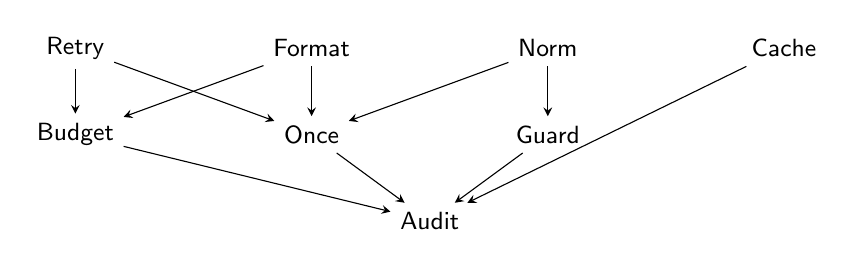
\begin{tikzpicture}[font=\small, >=stealth, node distance=1.1cm and 1.5cm]
  \node (retry) at (0,2.2) {\ly{Retry}};
  \node (format) at (3,2.2) {\ly{Format}};
  \node (norm) at (6,2.2) {\ly{Norm}};
  \node (cache) at (9,2.2) {\ly{Cache}};
  \node (budget) at (0,1.1) {\ly{Budget}};
  \node (once) at (3,1.1) {\ly{Once}};
  \node (guard) at (6,1.1) {\ly{Guard}};
  \node (audit) at (4.5,0) {\ly{Audit}};
  \draw[->] (retry) -- (budget);
  \draw[->] (retry) -- (once);
  \draw[->] (format) -- (budget);
  \draw[->] (format) -- (once);
  \draw[->] (norm) -- (once);
  \draw[->] (norm) -- (guard);
  \draw[->] (budget) -- (audit);
  \draw[->] (once) -- (audit);
  \draw[->] (guard) -- (audit);
  \draw[->] (cache) -- (audit);
\end{tikzpicture}
\caption{The relation for the eight layers that act on requests. An arrow from $x$ to $y$
says that $x$ must be above $y$. Arrows that follow from two others are left out.}
\Description{A diagram with Retry, Format, Norm and Cache in the top row, Budget, Once and
Guard in the middle row and Audit at the bottom. Arrows lead from Retry to Budget and Once,
from Format to Budget and Once, from Norm to Once and Guard, and from Budget, Once, Guard
and Cache to Audit.}
\label{fig:order}
\end{figure}

\paragraph{Eight layers.} For the eight layers of Table~\ref{tab:layers} that act on
requests, the relation has \exEightPairs{} pairs. \claim{eight-pairs}{They are the pairs of
Figure~\ref{fig:order} and those that follow from them.} \ly{Audit} is at the bottom, the
three layers that check stand below the layers whose moves their guarantees do not survive,
and \ly{Cache} is free above the log. Of the \exEightOrders{} orders, \emph{allowed} holds in
\exEightAllowed{}, \emph{covered} in \exEightCovered{}, \emph{within} in \exEightWithin{},
and \emph{exact} in \exEightExact{}. \claim{eight-orders}{All four hold in \exEightGood{}
orders, which is the number of linear extensions of the relation}, \exEightShare{} percent
of all. An order picked without thought is wrong for some guarantee almost always.
\claim{always-more}{With \ly{Always} in the place of \ly{Once}, the pair of \ly{Retry} and
the approval disappears and \exEightAlways{} orders are correct.}

\begin{table}
\caption{Every pair of the relation for the ten layers, with its two layers alone in the
wrong order, and the first scenario of the battery of Section~\ref{sec:eval} that breaks a
guarantee. The world shows what it received.}
\label{tab:witnesses}
\small
\begin{tabular}{llll}
\toprule
wrong order & the client asks & the world receives & broken \\
\midrule
\rows{witnesses}
\bottomrule
\end{tabular}
\end{table}

\paragraph{Ten layers.} With \ly{Redact} and \ly{Trim}, and a log that keeps the replies,
the relation has the cycle of Section~\ref{sec:up} and no order is correct. With a log of
requests the cycle is gone, \ly{Redact} must be below \ly{Trim} and \ly{Cache}, and
\exTenWeak{} of the \exTenOrders{} orders are correct, \exTenShare{} percent. The relation
with the full log has \exTenPairs{} pairs. \claim{witnesses}{Table~\ref{tab:witnesses} shows
each of them at work}: the two layers of a pair alone, in the wrong order, with a run that
breaks the guarantee. The table can be read as a list of the mistakes that a stack can make.

\begin{table}
\caption{Variants of the eight layers. The last column counts, over all stacks of five of the
ten layers, the guarantees that hold in every scenario although the relation says that they
can fail.}
\label{tab:variants}
\begin{tabular}{lrrr}
\toprule
variant & pairs & correct orders & hold against the relation \\
\midrule
\rows{variants}
\bottomrule
\end{tabular}
\end{table}

\paragraph{Variants.} The relation depends on details that look small.
Table~\ref{tab:variants} changes one at a time, recomputes Table~\ref{tab:survive} for the
changed world, and counts again. If the allow-list is closed under normalization,
\emph{allowed} survives the rewrite, the sandbox may stand above the hook that normalizes,
and more orders are correct. If the formatter is not in the allow-list, \emph{allowed} does
not survive the invented request, and fewer are. If a normal form can cost more than the
request, the budget must stand below the rewrite. \claim{variants}{In no variant does a
guarantee fail that the relation says holds. In one variant, the formatter outside the
allow-list, guarantees hold that the relation says can fail}, \exHiddenOutside{} of them over
the stacks of five: a \ly{Guard} below \ly{Format} drops the invented request, so that the
layers further down never see what \ly{Format} did. This is the incompleteness of
Theorem~\ref{thm:orders} again. A move of one layer is undone by another, and a relation
between pairs cannot see it.

\paragraph{Retries in several layers.} When more than one layer repeats, the repetitions
multiply. This is the retry storm of distributed systems, where a client, a gateway, and a
library each retry and a failing service receives the product~\cite{bronson2021}.

\begin{proposition}[Retries multiply]
\label{prop:multiply}
If every block of the layer $L_i$ has at most $m_i$ requests, then for one request of the
client the world receives at most $m_1 \cdots m_n$ requests. For layers that retry up to $t$
times the bound is reached when every call fails. A guarantee whose owner stands below every
layer that repeats holds however often they repeat.
\end{proposition}

\begin{proof}
By induction on $n$: the requests that reach $L_{i+1}$ for one request of the client are at
most $m_1 \cdots m_i$, and each has a block of at most $m_{i+1}$. A layer that retries $t$
times has a block of $t$ equal requests when all fail. The last sentence is
Theorem~\ref{thm:down}: no layer below the owner repeats.
\end{proof}

\begin{table}
\caption{One request of the client under layers that retry, when every call fails. The last
column has a budget of four below the retrying layers.}
\label{tab:retries}
\begin{tabular}{rrrr}
\toprule
layers that retry & tries each & requests at the world & with the budget below \\
\midrule
\rows{retries}
\bottomrule
\end{tabular}
\end{table}

\claim{retries-multiply}{Table~\ref{tab:retries} shows the product in runs, and the budget
that caps it.} The cap is the practical content of the affine mode: a budget at the bottom
needs to know nothing about the layers above it.

\section{Among the Correct Orders}
\label{sec:cost}

Correctness leaves \exEightGood{} orders of the eight layers, and they are not alike. Two
quantities differ between them that a user notices: how often the user is asked, and how
much of the budget is charged for requests that never reach the world. We ran every correct
order on the same \exWork{} random scenarios. The number of questions ranges from
\exAskedLeast{} to \exAskedMost{}, and the wasted budget from none to \exWasteMost{}.

The moves explain both numbers. A question is asked for every request that reaches
\ly{Once}. So every layer that drops and stands above \ly{Once} saves questions: the sandbox
refuses before the user is bothered, the cache answers before the user is bothered. Budget
is wasted for every request that \ly{Budget} has counted and that a layer below it drops. So
every layer that drops and stands below \ly{Budget} wastes budget. Both \ly{Once} and
\ly{Budget} are themselves layers that drop, and one of them is below the other.

\begin{table}
\caption{The correct orders of the eight layers that no other correct order improves in both
the questions to the user and the wasted budget, over \exWork{} random scenarios. The orders
are written from the top of the stack to the bottom.}
\label{tab:frontier}
\small
\begin{tabular}{rrrl}
\toprule
questions & wasted & orders & one of them \\
\midrule
\rows{frontier}
\bottomrule
\end{tabular}
\end{table}

Table~\ref{tab:frontier} lists the \exFrontier{} combinations of the two numbers that no
correct order improves in both. \claim{frontier}{No order is best in both. The orders that
waste nothing have \ly{Once} above \ly{Budget}, and all others on the list have \ly{Budget}
above \ly{Once}.} With \ly{Budget} at the bottom, just above the log, nothing that it counts
is dropped, and the user is asked about requests that the budget then refuses:
\exAskedNoWaste{} questions. With \ly{Once} at the bottom the user is asked least,
\exAskedLeast{} times, and \exWasteLeastAsked{} units of budget are charged for requests that
a layer below the budget then drops. Which is better depends on what is scarce, the attention of the user or
the budget, and the account of moves says what each choice costs before the stack is built. In
all orders of the list the sandbox and the cache stand above whichever of the two is lower.

\section{Evaluation}
\label{sec:eval}

The artifact is one Python script of about \exLines{} lines with no dependencies; its random
choices come from one generator with seed \exSeed{}. It
implements the ten layers of Table~\ref{tab:layers} and the layer \ly{Always} over a small
world: a file with a version, a file whose content starts with a secret, a secret file
outside the sandbox, a path that is spelled inside the sandbox and normalizes to that file, a
long page, and a formatter. A scenario fixes what the client asks for, which calls of the
world fail, what the user answers, and the numbers $B$, $N$, and the number of tries. A run
records the calls of the world, the letters of the layers, the replies to the client, and the
block of every request at every layer. The command \texttt{make -C artifact check} runs the
script and compares its output with the files from which this paper takes its numbers and
the rows of its tables.

\paragraph{The prediction.} The script holds the two tables: what each layer does
(Table~\ref{tab:layers}) and what each guarantee survives (Table~\ref{tab:survive}), the
latter computed. From them it predicts, for a stack and a guarantee, whether the guarantee
holds in every run, by Definition~\ref{def:above}.

\paragraph{The observation.} A battery of \exBattery{} scenarios makes every layer do what
it can do: the cache answers, a call fails and is retried under a tight and under a wide
budget, a request is rewritten to an allowed one, under a wide and under a tight budget, and to a
forbidden one, the guard, the user,
and the budget each refuse, the formatter runs, a reply carries a secret, and a reply is
long. A guarantee is observed to hold for a stack if it holds in all runs of the battery.

\paragraph{Every order.} \claim{eight-agree}{For each of the \exEightOrders{} orders of the
eight layers that act on requests, prediction and observation agree on every guarantee.}
\claim{fives-agree}{They also agree for all \exFives{} stacks that consist of five of the
ten layers in some order, with \exFiveGuarantees{} guarantees between them, for the log in
both forms, and for \exTens{} random orders of all ten layers with \exTenGuarantees{}
guarantees.} Agreement has two directions. Where the theory says that a guarantee holds, no
scenario violates it. Where the theory says that it can fail, some scenario of the battery
violates it. The second direction is the one that Theorem~\ref{thm:orders} does not promise:
for these layers and scenarios no move is hidden. The first direction is tested further.
\claim{sound}{In \exSoundRuns{} runs of random stacks under random scenarios, with random
clients, failures, answers of the user, and numbers, the \exKept{} guarantees that the
theory says hold all hold.}

\paragraph{Deliberate mistakes.} The script has \exMutants{} switches that each plant one
mistake: \ly{Retry} or \ly{Cache} is said to do nothing; \emph{allowed} is said to survive
the rewrite, \emph{within} to survive $\rep$, or \emph{covered} to survive the invented
request; \ly{Redact} is said to keep shortness; the log is said to be clean wherever it
stands; the direction is confused, so that the layers above the owner are examined instead
of those below; and one layer, \ly{Budget}, is made to send every request twice while the
table still says that it only drops. \claim{all-noticed}{Each is noticed}: the first eight
by a disagreement between prediction and observation, the last by the check of the blocks.

\paragraph{What the tests do not show.} The agreement is for ten layers that we wrote, with
a world of six objects. It shows that the two tables predict these layers on every order,
and not that every layer of a real harness can be described by four moves. The battery was
written with the moves in mind, and we know of one case that it would miss if it had only a
tight budget: the masked violation of Section~\ref{sec:orders}.

\section{Related Work}
\label{sec:related}

\paragraph{Where a function belongs.} The end-to-end argument~\cite{saltzer1984} says that a
function such as reliable delivery cannot be completed by a layer in the middle and belongs
at the ends; the principle of complete mediation asks that every access be
checked~\cite{saltzer1975}. Both are advice about one function. Our relation says, for many
functions at once, which must be nearer to the world than which, and the two tables say why.
Layered systems were built from reusable layers in the x-kernel~\cite{hutchinson1991} and in
Click~\cite{kohler2000}, and \citet{batory1992} gave layers types that say which
compositions are meaningful. \citet{eriksen2013} describes the filters of a service as
functions on services and composes timeouts, retries, and authentication by function
composition, in an order that the programmer chooses. In telecommunications, features that interact are ordered by a precedence
relation that the designers supply~\cite{jackson1998}. We derive the relation.

\paragraph{Aspects and the properties that they preserve.} The closest work is on aspects.
\citet{rinard2004} classify advice by whether it runs the code that it wraps once, not at
all, or several times, and by what it reads and writes. \citet{katz2006} sorts aspects into
categories and shows for each which classes of temporal properties of the base program it
preserves, and \citet{djoko2012} define categories by syntax and prove the preservation.
\citet{dantas2006} give a type system for advice that cannot change the result of the code
that it advises. \citet{douence2004} detect interactions between aspects that apply at the
same point and let the programmer resolve them. Our moves are a classification of this kind,
and Theorem~\ref{thm:down} is a preservation result. The differences are the object and the
question. A stack has an order and two directions, each layer is at once something that
preserves and something whose guarantee must be preserved, and the question is which orders
are correct. The answer by modes and patterns, the cycle, and the comparison on every order
are new as far as we know.

\paragraph{Effects.} Layers are the handlers of an effect of calling the world, and the
order of handlers matters as the order of monad transformers
does~\cite{liang1995,plotkin2009,kammar2013}. The algebraic account of when effects can be
combined without regard to order is the tensor of theories~\cite{hyland2006}. That work asks
when two orders give the same program. We ask the weaker and more practical question
whether an order keeps stated guarantees, which two orders that differ as programs may both
do: \ly{Once} above \ly{Budget} and \ly{Budget} above \ly{Once} ask the user a different
number of questions and keep the same guarantees.

\paragraph{Substructural modes and well-quasi-orders.} The structural rules and the modes
that their absence defines come from linear logic~\cite{girard1987}, and graded type systems
refine the modes to counts~\cite{orchard2019}. Monitors that stop executions enforce safety
properties~\cite{schneider2000}; the layers that drop are monitors of this kind. That languages
closed under leaving out letters are regular is due to \citet{haines1969}, by the lemma of
\citet{higman1952}. We use it to give the affine guarantees a finite form, and the test for
repeated letters seems to be new in this role.

\paragraph{Agents.} The layers are those of the earlier papers of this series taken
together: approvals~\cite{tpp4}, budgets for cost~\cite{tpp6}, gates for untrusted
text~\cite{tpp7}, retries and journals~\cite{tpp8}, and the ledger of
obligations~\cite{tpp12}, which is a layer that drops. Each of those papers studies one layer
on its own. This one is about putting them in one stack. The practice of binding every number
to the script and marking the sentences that the script checks follows~\cite{tpp10}.

\section{Limits and Conclusion}
\label{sec:limits}

\paragraph{Limits.} The model is synchronous and sequential. Layers that act later, such as
a queue that batches requests or a timeout that gives up on a call that is still running,
change the order of requests, which is a fifth move that we do not treat. The relation is
sound and not complete, as the masked case shows, and it compares layers pairwise: a layer
that undoes the move of another, such as a journal that removes the repetitions of a retry,
needs an account of what a group of layers does together. A rewrite is described by a
function, and a guarantee survives it or not as a whole; a rewrite that is harmless for some
requests is treated as harmful. The characterization by patterns covers guarantees over
requests alone. And the evaluation is on layers that we wrote.

\paragraph{Conclusion.} A layer is correct at its own edge, and a stack is correct when each
guarantee survives the rest of the way. What survives what can be tabulated, the tables
decide the orders, and for the layers of an agent harness \claim{one-in-hundred}{the correct orders are less
than one in a hundred}. The remaining choice is not where to put the layers. It is which
guarantees to ask for: what a yes of the user covers, and whether a log should be exact or
safe to keep.

\bibliographystyle{ACM-Reference-Format}
\bibliography{refs}

\end{document}
